\documentclass[10pt,twocolumn]{IEEEtran11}

\usepackage{times}
\usepackage{epsfig}
\usepackage[T1]{fontenc}
\usepackage{graphicx}
\usepackage{subfigure}
\def\BibTeX{{\rm B\kern-.05em{\sc i\kern-.025em b}\kern-.08em
    T\kern-.1667em\lower.7ex\hbox{E}\kern-.125emX}}

\oddsidemargin -15pt
\evensidemargin -15pt
\leftmargin 0 pt
\topmargin -30pt
\textwidth = 6.9 in
\textheight = 9.0 in

\newcommand{\itembase}{\setlength{\itemsep}{0pt}}
\newcommand{\eg}{{\it e.g., }}
\newcommand{\ie}{{\it i.e., }}
\graphicspath{{FIG/}}

\begin{document}

\bibliographystyle{IEEE}

\title{\Large \bf A Comparison of Distributed Data Processing Systems}
\author{
Vincent M Chen\\
Information and Computer science Department\\
University of Oregon\\
{\em applekey@cs.uoregon.edu}
}
\maketitle

\section{Introduction}
The explosion of data in the past decade has lead to many questions in finding the most efficient method in order to analyze the data being generated. Best put by Google's CEO, Eric Schmidt, "There were 5 exabytes of information created by the entire world between the dawn of civilization and 2003. Now that same amount is created every two days.", more precisely, in 2003, 6.8 exabytes were being created every 2 days,\cite{gantz2010digital}.  With such a large volume of throughput, trivial tasks such as locating a users' account or finding all users within the same group can't be found in meaningful time with a single computers nor using sequential algorithms.
\par
In order to solve this problem, a very important insight is to notice that a large majority of the data being created is independent from each other, ex. different users on an on-line shopping platform where every shopper has their own independent profile, shopping cart and payment information.  Independence within the data means that parallel computation can be used, where instead of a single computer processing data sequentially, the job is divided into many sub tasks and processed in parallel.  This allows the computation of a large data set to be divided among the processing power of multiple computers.
\par
These parallel computation systems have existed since the 1980's, the most common of which are database systems. In the time since, many database systems have evolved into both parallel and distributed varieties.  As well, alternative computation frameworks introduced recently such as map reduce or Apache Spark have taken a  similarly approach to that used by databases, parallel computation.  The goal of this survey paper is to firstly introduce these different data query systems and their variants.  Secondly, discuss the common approaches all of them use to speed up computation and finally highlight unique aspects of each system.

\section{Basic Description of Functionality}

A data processing solution should satisfy the following functionality:
\begin{enumerate}	
	\item Guarantee high degree of fault tolerance.
	\item Compute a user defined query in a reasonable time.
\end{enumerate}

\subsection{Fault Tolerance}
Fault tolerance is the most important guarantee that a computation framework provides.  Without consistency, the data being returned from the query cannot be used for any meaningful analysis. Fault tolerance means recovery from failure from multiple sources

\begin{enumerate}
	\item Network fault, communication between compute nodes is unreliable and data is lost in between
	\item System fault, OS failure
	\item Hardware fault, compute computer hard disk fails
	\item User fault, user query has code that leaves query engine in a bad state
\end{enumerate}

In order for user defined queries to complete in a reasonable time, two levels of parallelization can be applied.

\subsection{Parallel Computation}
The framework can process independent queries in parallel.  For example, searching for all students who owe more than 10,000 dollars in student loans
can be queried in parallel, each student can be treated independently.

\subsection{Distributed Computation}
The framework is able to distribute the data set across multiple compute machines.  Each machine might contain independent data, for example, one machine contains all students with first names starting A to J and another from K to Z.  Another case is multiple machines hold data that is related to one another.  For example in figure \ref{fig:distDataDependency}, machine A might hold all student's GPA and Awards and another machine holds the student's student loan amount.
If the query were to find all students that had more than 10,000 in student loans but also a 4.0 GPA in order to give them a financial award, then each query per student would need to look at the data in both compute machines.

\begin{figure}[h]
\centering
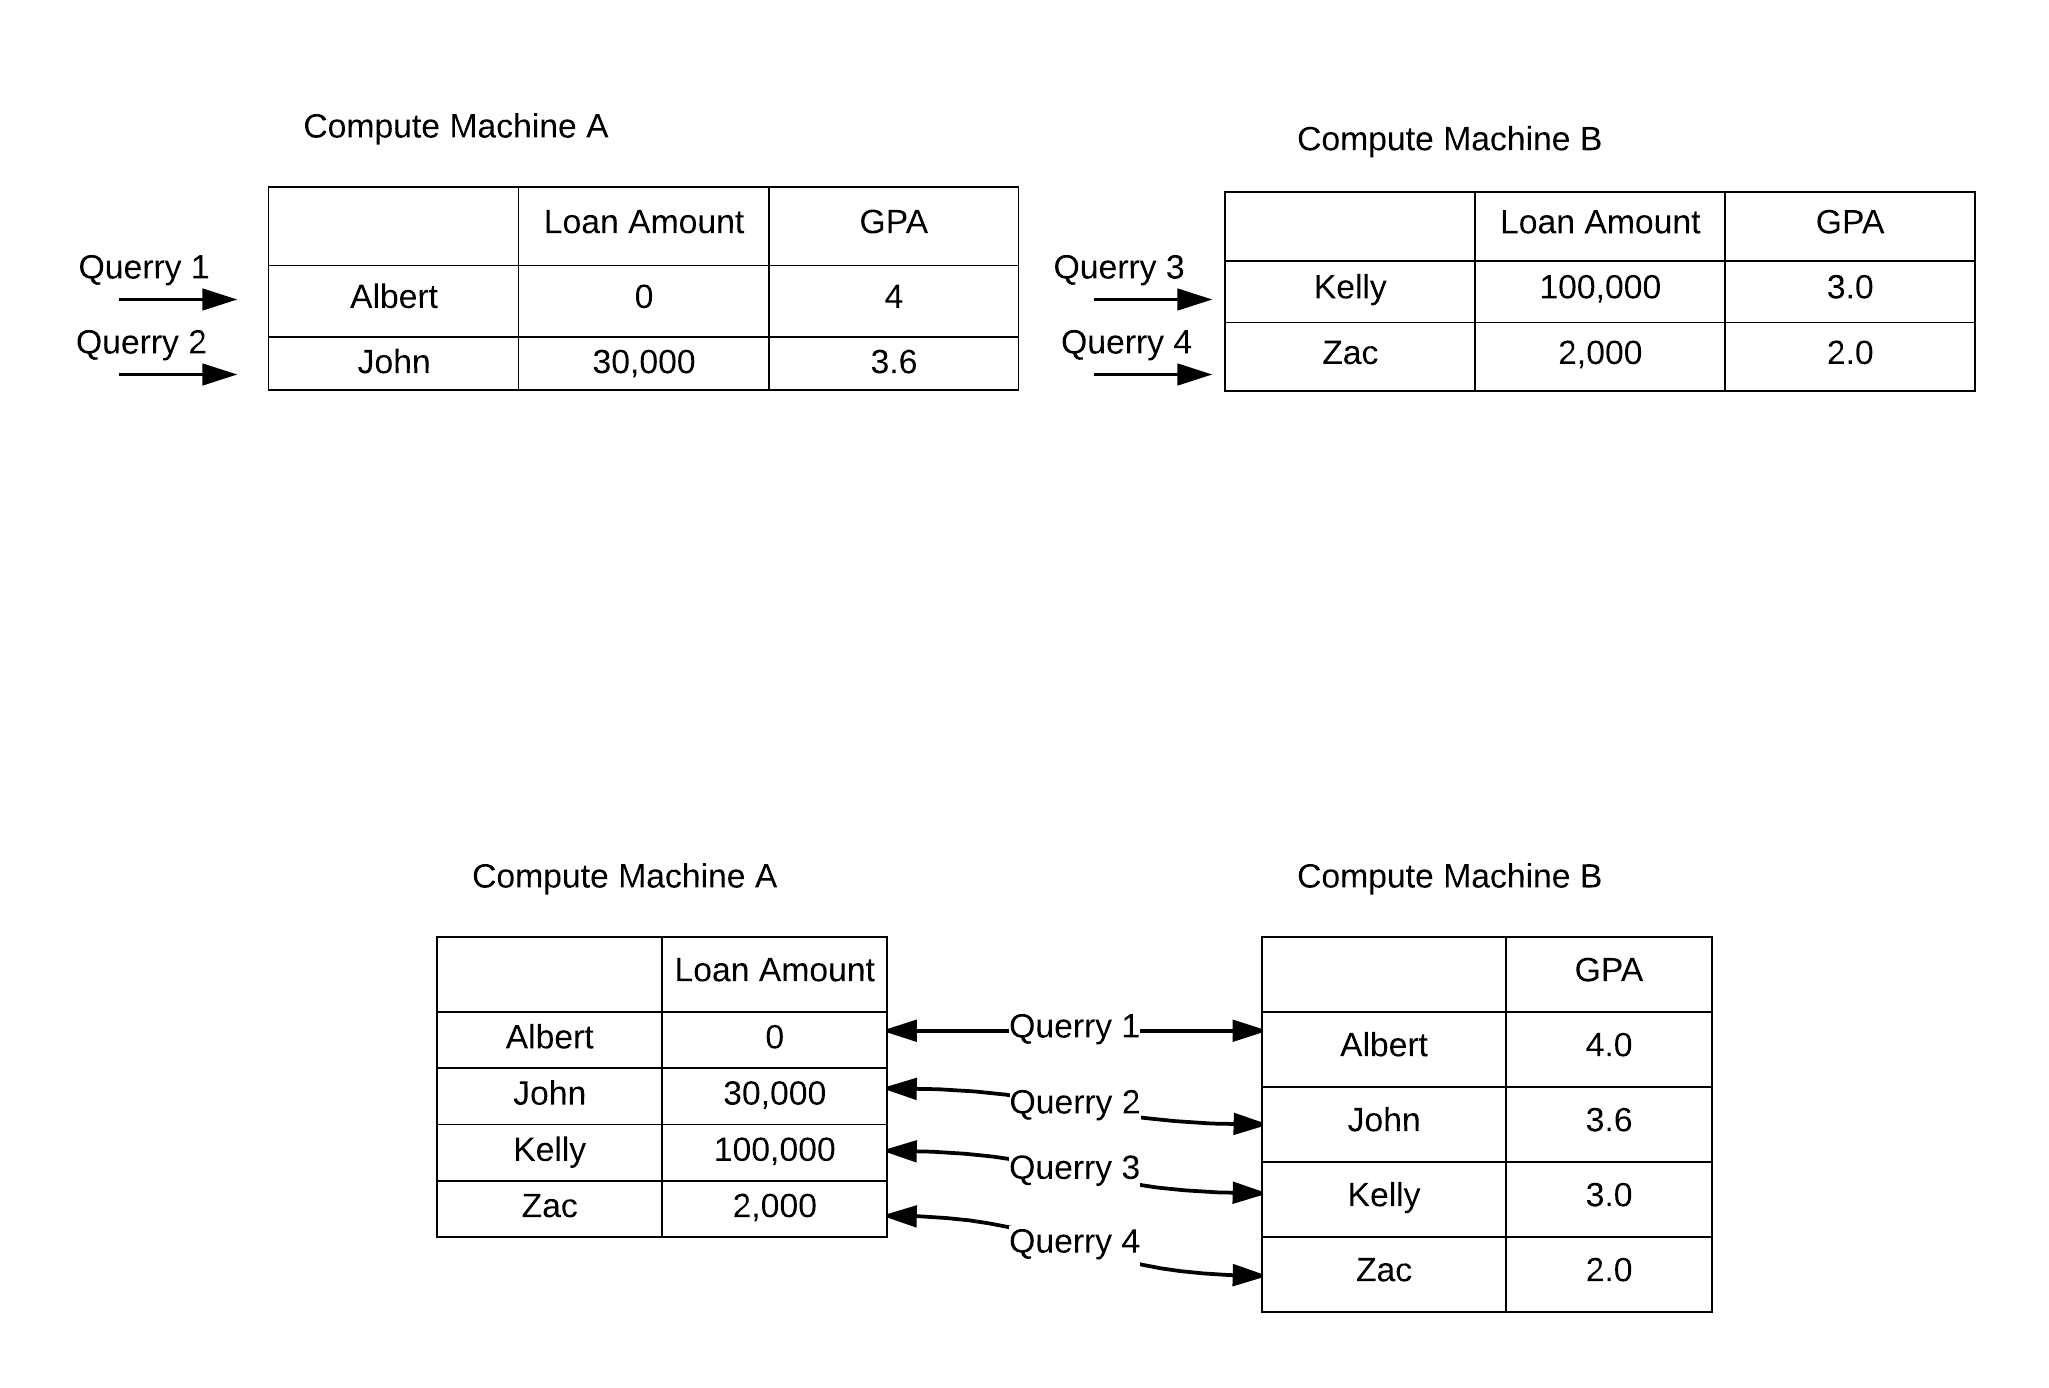
\includegraphics[scale=0.12]{images/parallelComputation.png}
\caption{Distributed Data Dependency}
\label{fig:distDataDependency}
\end{figure}

\section{Databases Management Systems}

Databases management systems are  frameworks that are designed to store data in tabular tables with a set schema.  DBMS systems use relational queries to perform CRUD 
(Create, read, update and delete)operations on the stored data.  

%%\fix{write more here}

\subsection{Parallel DBMS}

Relational queries are ideal suited to run parallel since they
each operation declares independent operations on independent data sets \cite{dewitt1992parallel}.  By partitioning the data among multiple processors, a single query can be carried out in parallel and the result merged into a final step.  In figure \ref{fig:disDBMS}, an independent scan (ex, look for key word) is applied and the results are sorted (binned by first letter) and then the result of each independent operation is merged into the final result.

\begin{figure}[h]
\centering
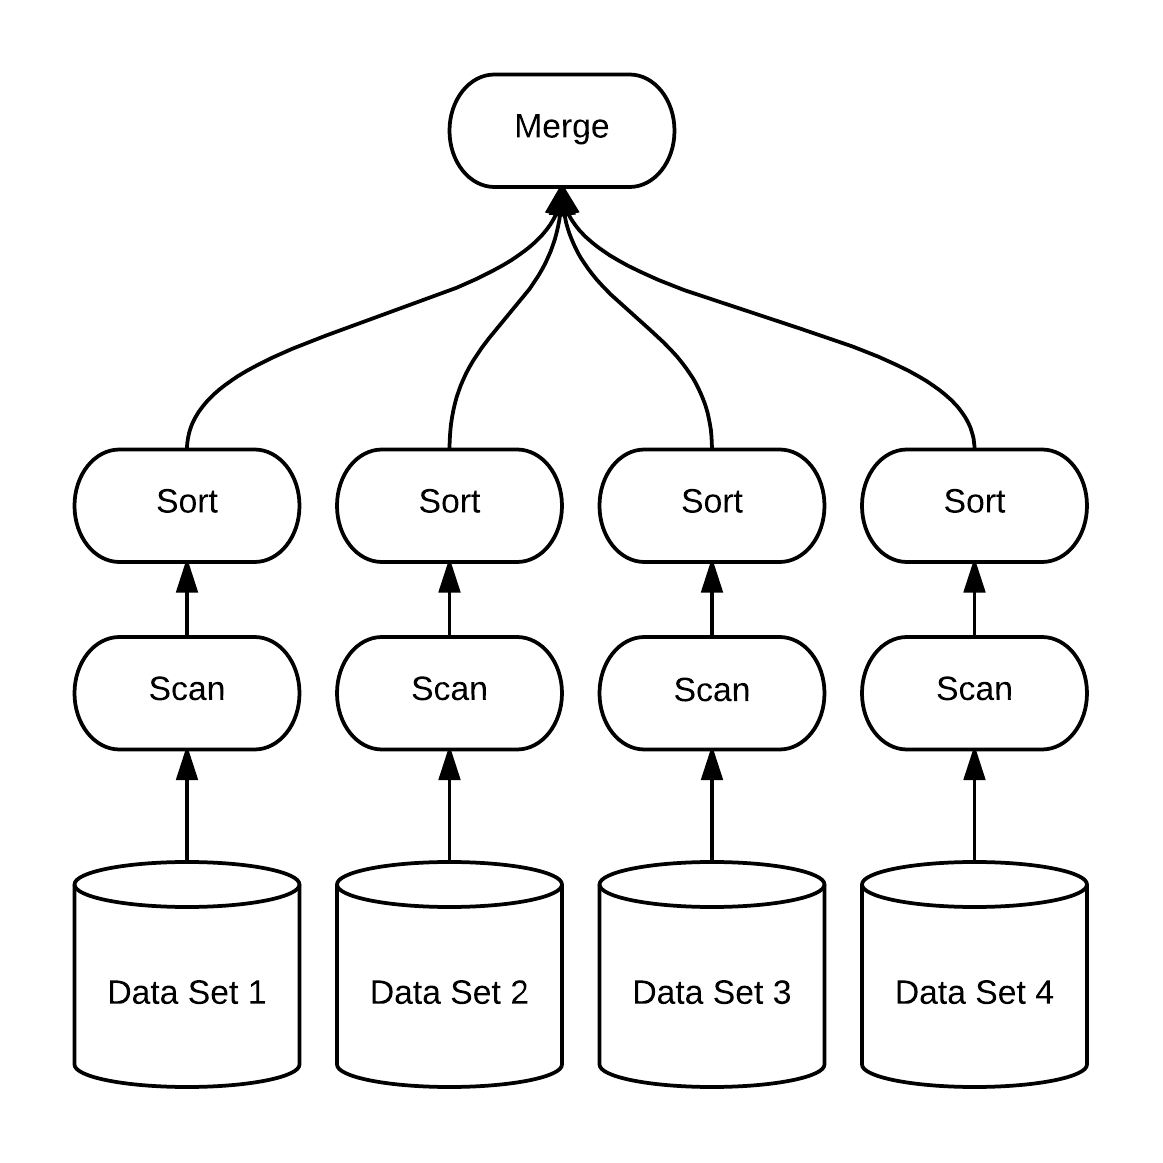
\includegraphics[scale=0.12]{images/parDBMS.png}
\caption{Distributed Data Dependency}
\label{fig:disDBMS}
\end{figure}

\subsection{Distributed DBMS}

Distributed DBMS systems require an additional layer of abstraction on top of Parallel DBMS.  Where as in parallel DBMS systems, all queries are run on the same machine sharing the same memory space.  Distributed DBMS systems need to consider the additional factor of latency when access data that does not reside in the current compute machine.  Additional, distributed DBMS systems need to consider what impact does the memory layout have in preventing easily adding more compute nodes.  

Generally speaking, there are three main types of memory 
architectures for distributed DBMS systems, shared-nothing, shared-memory, shared-disk.

\begin{enumerate}
\item Shared-Memory: All compute machines share access to a global memory as well as disk storage.  
\item Shared-Disk: Each compute machines have their own memory, but share global disk.
\item Shared Nothing: Each compute machine has their own memory and disk. 
\end{enumerate}

\subsection{Fault Tolerance}


\section {Map Reduce}

Map Reduce is a general distributed computation framework introduced by Google in 2004 \cite{dean2001mapreduce}.  Map reduce is different from distributed DBMS systems in that much more general computations can be defined, not limited by the query language of a rigit schema as is the case with DBMS systems.  Map Reduce, like DBMS systems have fault tolerance mechanisms but they operate differently than DBMS systems due to the architectural differences. 

\subsection{Mapper and Reducer}
Map reduce operates in two steps, the map step and then the reduce step.  Both steps are independent in that the reduce step will not start until all mappers have completed.
In the map stage, the data is partitioned equally among N mappers.  Input data arrives to the mapper as a list of (key, value) pairs, the mapper applies a user-defined map operation.
The map operation produces intermediate (key, value) pairs which are the results of the map operations.  
\par
The reducer is again a user defined operation that processes the intermediate values from the mapper grouped by key.  The reducer can produce zero or an aggregate of all values
that map to the same key.

Figure \ref{fig:mapReduce} gives an execution diagram.
\begin{figure}[h]
\centering
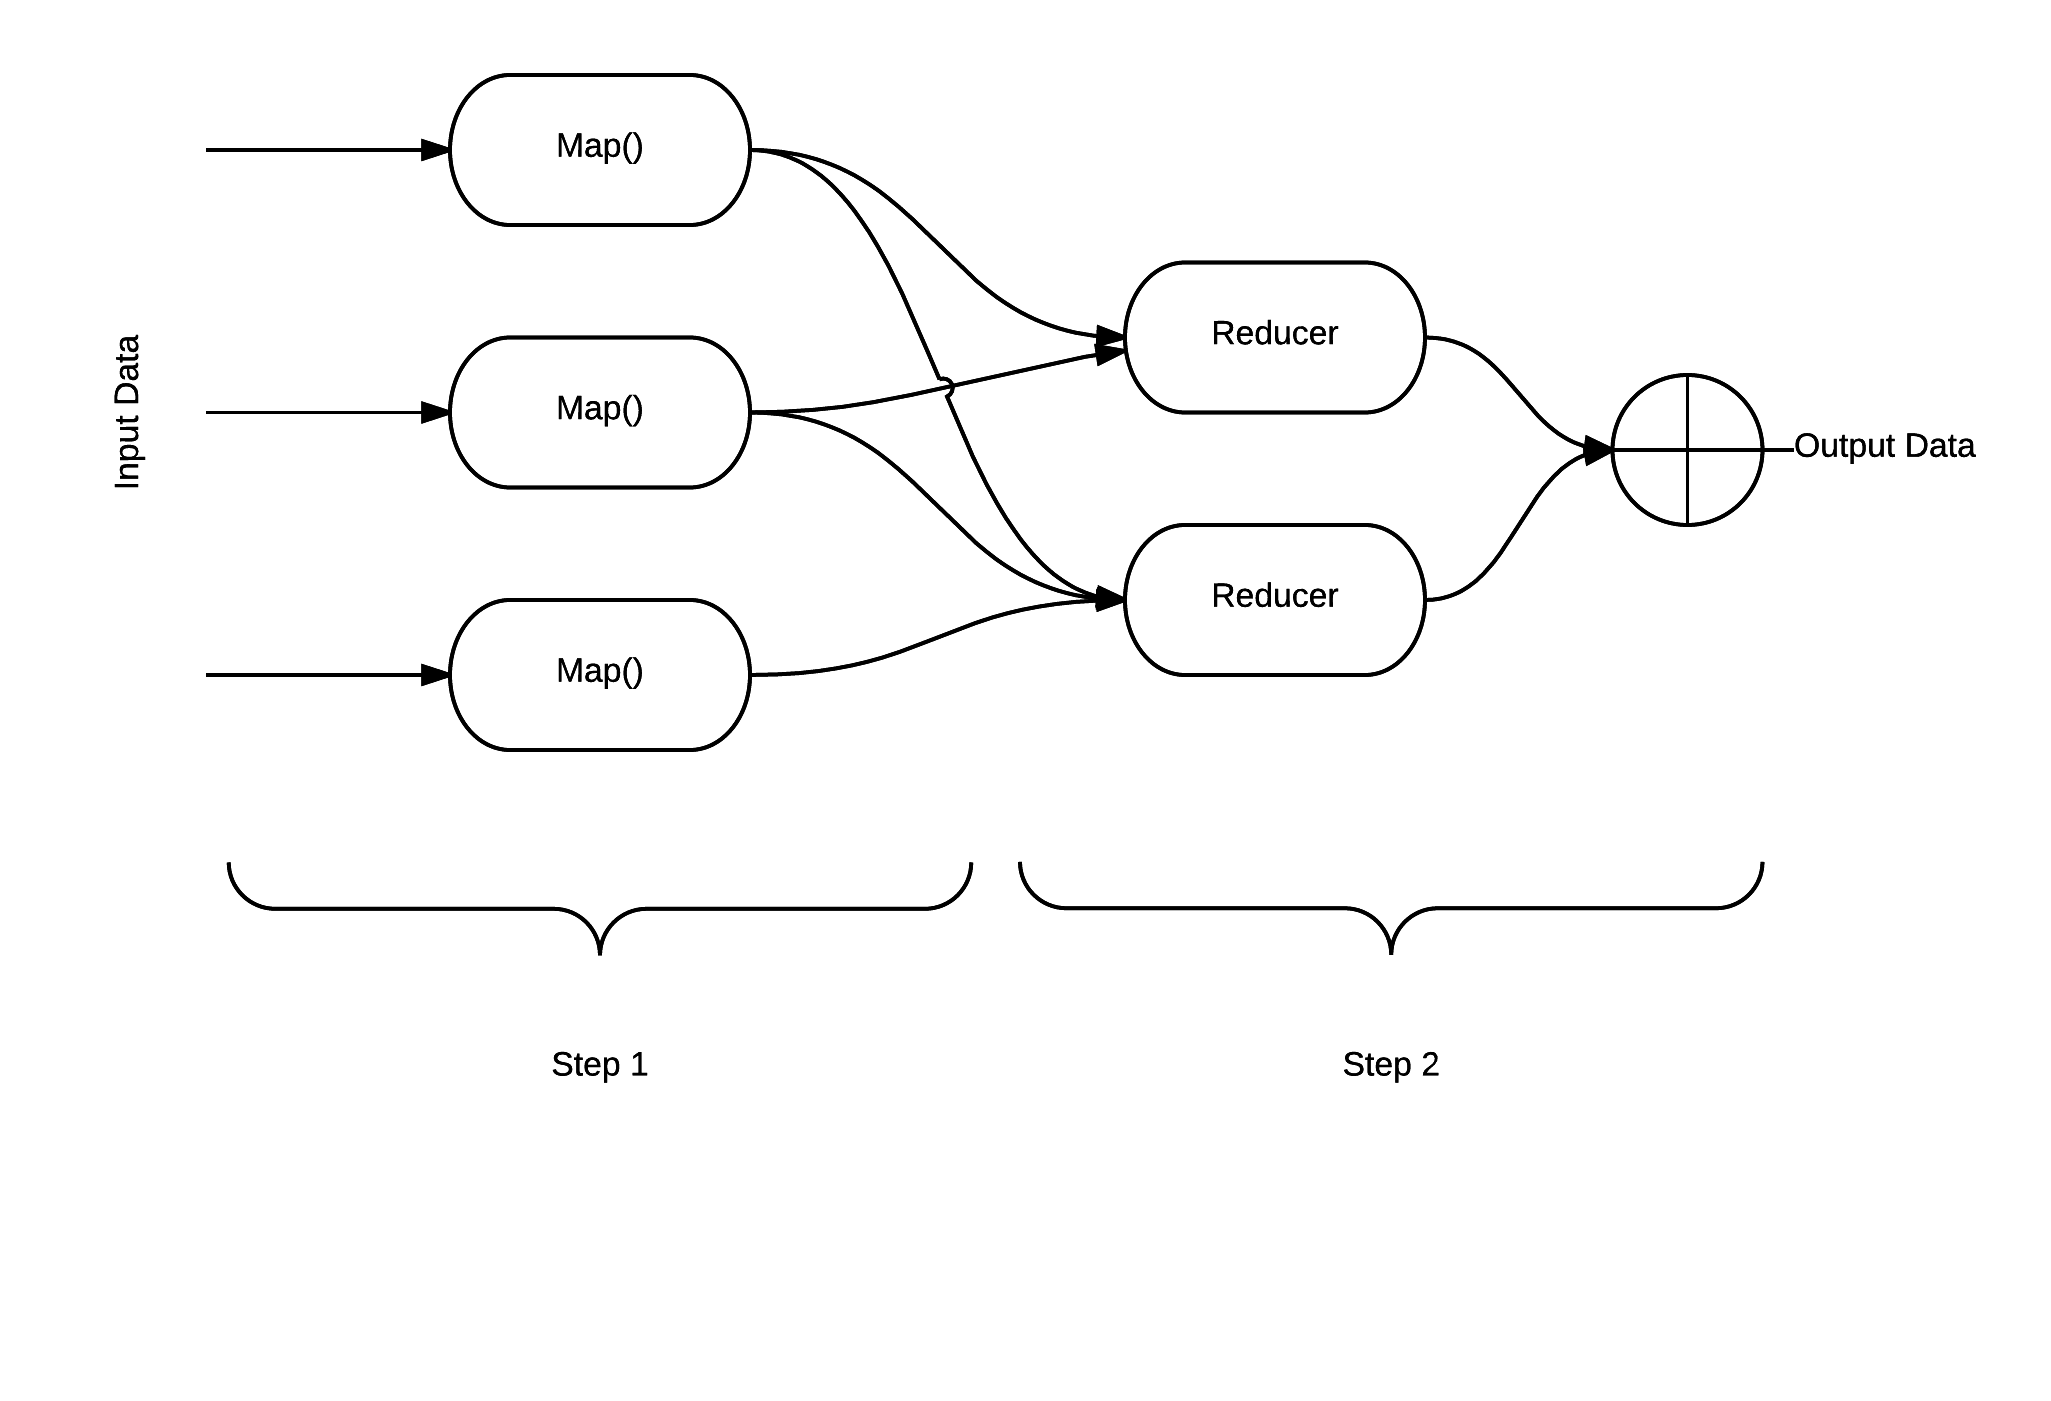
\includegraphics[scale=0.50]{images/mapReduce.png}
\caption{Map Reduce Program Execution}
\label{fig:mapReduce}
\end{figure}

\subsection{Hadoop}
There are two very popular frameworks that implement the map reduce concept, these are the closed source Google Map Reduce and open source version Hadoop Map Reduce.  
This paper will focus on Hadoop instead of Google Map Reduce since the complete details of Google Map Reduce and relatively unknown, however both frameworks function similarly.
\par
Hadoop consist of three layers:
\begin{enumerate}
	\item Application layer
	\item Map Reduce layer
	\item HDFS layer
\end{enumerate} 




\subsection{Fault Tolerance}





Analgous to parallel DBMS, the map and reduce step are very similar to a filter and reduce.

























\bibliography{citations}


\end{document}
